\chapter{Methodology}
This research investigates if trajectory optimisation can be used to inspire controller design for a bipedal pneumatic-electrical robot on different terrains. 

\textbf{THIS NEEDS TO BE FILLED OUT SOME MORE}

\section{Modelling and Simulating the System} \label{model}
This section of the research covers the following three main aspects. Namely: the mathematical modeling of the system to obtain the equations of motion (EoM), generating trajectories to analyse using trajectory optimisation and lastly, to use these trajectories to aid in the design of controllers. These methods are described in more detail in the relevant sections down below.

%%%%%%%%%%%%%%%%%%%%%%%%%%%%%%%%%%%%%%%%%%%%%%%%%%%%%%%%%%%%%%%%%%%%%%%
    \subsection{Equations of Motion} \label{dynamics}
    The equations of motion (EoM) were generated using the manipulator equation that look as follow \cite{Robotics-2010, Underactuated-2022}:
    
    \begin{equation} \label{eq:eom}
        \bm{M}(\bm{q})\ddot{\bm{q}} + \bm{C}(\bm{q},\dot{\bm{q}})\dot{\bm{q}} + \bm{G}(\bm{q}) = \bm{B}\bm{\tau} + \bm{A}\bm{\lambda}
    \end{equation}
    
    Where $\bm{M}$ is the mass matrix, $\bm{C}$ the Coriolis matrix, $\bm{G}$ the gravitational potential matrix, $\bm{B}$ maps the applied forces and torques to the generalised coordinates and $\bm{A}$ the external forces to the generalised coordinates. $\bm{q}$ is the generalised coordinates of the robot and was changed depending on the model being used. for fixed-body the model was the following:
    
    \begin{equation}
        \bm{q} = [x,z,\theta_{\textit{leg left}}, \theta_{\textit{leg right}}, r_{left}, r_{right}]^T
    \end{equation}
    
    The generalised coordinates for the free-body looks as follow:
    
    \begin{equation}
        \bm{q} = [x,z, \theta_{body},\theta_{\textit{leg left}}, \theta_{\textit{leg right}}, r_{left}, r_{right}]^T
    \end{equation}
    
    $\tau$ defines the applied forces acting on the robot. The robot model consists of a motor attached at the hip and a pneumatic actuator acting as the leg, this was the case for both of the legs. There is also a damping applied in the $x$-direction to compensate for the friction acting in on the support rig (more about the rig in Chapter \ref{robot}), the force matrix looks as follow:
    
    \begin{equation}
        \bm{\tau} = [-b\dot{x}, F_{\textit{applied left}}, F_{\textit{applied right}}, \tau_{\textit{hip left}}, \tau_{\textit{hip right}}]^T
    \end{equation}
    
    Where $-b\dot{x}$ represents the damping applied on the robot due to the friction acting on the support rig. Where $F_{applied} = F_{applied}^{extend} - F_{applied}^{retract} - F_{reaction}^{extend} + F_{reaction}^{retract} - b\dot{r}$ and looks the same for $F_{\textit{applied left}}$ and $F_{\textit{applied right}}$. The forces, $F_{applied}^{extend}$ and $F_{applied}^{retract}$ represents the prismatic actuation force of the pneumatic cylinder and was separated into extension and retraction to allow complementarity constraints to be applied, this is discussed in more detail in Section \ref{Bang-Bang}. The forces, $F_{reaction}^{extend}$ and $F_{reaction}^{retract}$ represents the hard stop forces that acts on the cylinder when it reaches its extension and retraction limits, discussed in more detail in Section \ref{Hard Stops}. Lastly, $\tau_{hip}$ are the forces applied by the servo motors at the hip.
    
    The external forces, $\lambda$, in Eq. \ref{eq:eom} were just the ground reaction forces. This is due to the only working in the sagittal plane. The forces were represented as follow:

    \begin{equation} \label{eq:GRF}
        \bm{\lambda} = [\lambda_x^+ - \lambda_x^-, \lambda_z]^T
    \end{equation}
    
    The forces $\lambda_x$ and $\lambda_y$ are the ground reaction forces. The force along the $x$-axis was split into a positive and negative force, this was done for the purpose of complementarity constraints and is explained in more detail in Section \ref{through-contact}.
    
    The EOMs are described as an equation and is implemented as a constraint in the trajectory optimisation. Further details on how the EOMs were generated can be found in Appendix \ref{app-a}.
    
    %%%%%%%%%%%%%%%%%%%%%%%%%%%%%%%%%%%%%%%%%%%%%%%%%%%%%%%%%%%%%%%%
    \subsection{Trajectory Optimisation}
    Trajectory optimisation is a set of mathematical tools that are used to generate a trajectory that minimises a measure of performance, cost function, that satisfies a number of constraints and variable bounds \cite{Fisher-2020}. The trajectory is divided into $N$ node points. Constraints are applied to ensure a feasible transition between nodes. Bound are set to narrow down the search space for a feasible solution. The constraint are satisfied by varying the decision variables between the their bound until a feasible and optimal solution is found.
    
    Due to the fact that the problems that are being optimised are complex, there is no guarantee that the solver will find an optimal solution on the first attempt. To increase the likelihood that the solver to solver will find an optimal solution, multiple optimisation are usually ran from different randomly generated seed point, start point of the optimiser, using uniform random distributed numbers between the variable bound. This also leads to the solver exploring more of the search space.
    
    There are numerous cost functions that exist but the one that was used to generate the trajectories looks as follow: 
    
    \begin{equation} \label{eq:cost}
        J = \sum^N_{i=1} (\tau_{Right}(i)^2 + \tau_{Left}(i)^2)
    \end{equation}
        
    $J$ is the cost function which aims to minimise the absolute torque the hip motors use throughout the trajectory. With $\tau_{Right}(i)$ being the right hip's motor torque at the $i^{th}$ node point and with $\tau_{Left}(i)$ being the left hip's motor torque at the $i^{th}$ node.
    
    \textbf{PLEASE ADD MORE TEXT DEVLON}
    
    %%%%%%%%%%%%%%%%%%%%%%%%%%%%%%%%%%%%%%%%%%%%%%%%%%%%%%%%%%%%%%%%%%%%%%%%%%%%%5
        \subsubsection{Collocation}
        A trajectory is split up into $N$ finite elements (node point, designated as $i$) which describes the motion of each generalised coordinate along the path. The trajectory between each node if further split into more points using a Runge-Kutta basis with 3 collocation points as can been seen in Figure \ref{fig:collocation}, designated as $j$. Thus, the trajectory was divided into $N$ node points, $i\in[1,N]$, each with 3 collocation point in between, $j\in[1,3]$. Additional constraints were placed to ensure that the last value of the collocation point lines up with the value of the upcoming node, this was done to ensure a smooth trajectory and this can be seen in Figure \ref{fig:collocation} \cite{Fisher-2020}. Three point Radau was used to solve the differential equations in Section \ref{dynamics}, at selected time points \cite{Fisher-2020}. This was done by implementing the following equations:
        
        \begin{figure}[ht!]
            \centering
            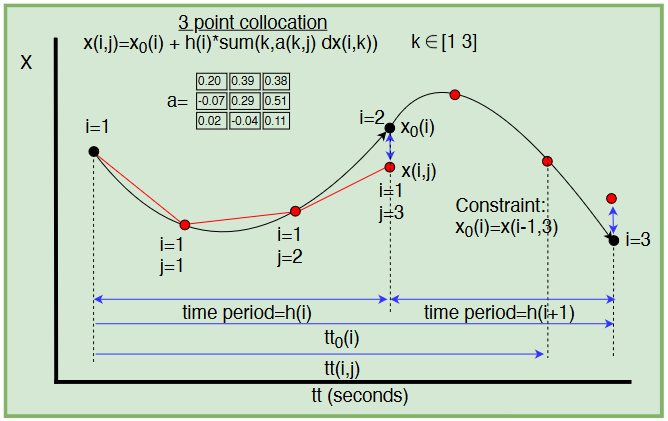
\includegraphics[width=\textwidth]{figs/collocation}
            \caption{Shows a graphical representation of how the trajectory is broken up into node points ($i$) and collocation points ($j$). Additional constraints are also shown.}
            \label{fig:collocation}
        \end{figure}
        
        \begin{equation} \label{eq:collocation}
            \begin{split}
                \bm{q}(i,j) & = \bm{q}_0(i) + h(i) \times \sum_{k=1}^{3} \bm{a}(k,j)\dot{\bm{q}}(i,k) \\
                \dot{\bm{q}}(i,j) & = \dot{\bm{q}}_0(i) + h(i) \times \sum_{k=1}^{3} \bm{a}(k,j)\ddot{\bm{q}}(i,k) \\
                \bm{q}_0(i) & = \bm{q}(i - 1,3) \\
                \dot{\bm{q}}_0(i) & = \dot{\bm{q}}(i - 1,3)
            \end{split}
        \end{equation}
        
        The equations in Eq.\ref{eq:collocation} were implemented for each state trajectory ($\textbf{q}$ and $\dot{\textbf{q}}$). The first two equation implement the three point Radue to integrate the state trajectories from the node $i$ to $i+1$, whereas the last two equations ensure that last collocation point of node $i$ is located at the same point as node $i+1$ and this ensures a continuous smooth trajectory. The difference between $\textbf{q}(i,j)$ and $\textbf{q}_0(i)$ is that $\textbf{q}(i,j)$ acts on node point ($i$) and collocation point ($j$), whereas $\textbf{q}_0(i)$ only acts on the node point ($i$). The three point collocation matrix that was used in Eq.\ref{eq:collocation} looks as follow \cite{Fisher-2020}:
        
        \begin{equation} \label{eq:3p_matrix}
            \bm{a} = \begin{bmatrix}
                0.19681547722366 & 0.39442431473909 & 0.37640306270047 \\
                -0.06553542585020 & 0.29207341166523 & 0.51248582618842 \\
                0.02377097434822 & -0.041548752126002 & 0.11111111111111 
            \end{bmatrix}
        \end{equation}
        
        For the model that was used contacts were required to occur at node points and not in-between them, a variable time-step was required for this. A variable time-step allows the optimiser to increase the resolution at critical points (such as contact events) as well as decrease the resolution at less critical points (for example the aerial phase). The time-step between each element is constrained as follow:
        
        \begin{equation} \label{eq:time_step}
            \begin{split}
                0.25h_M &\leq h(i) \leq h_M \\
                tt(i,j) &= tt_0(i) + h(i) \sum^3_{k=1} \bm{a}(k,j) \\
                tt_0(i) &= tt(i - 1,3)
            \end{split}
        \end{equation}
        
        $h(i)$ is the time-step for the $i^{th}$ node point and was bound between $h_M$ and $0.25h_M$, this was set according to the expected time the task will take to complete. $tt$ is the total time from the start of the trajectory to the relevant node ($i$) and collocation point ($j$). The first equation in Eq.\ref{eq:time_step} bounds the time-step between a minimum and maximum value, the second equation splits up the node time among the collocation points and the third equation ensures that the start time of the $i^{th}$ node, $tt_0(i)$, matches the end time of node $i-1$ at the third collocation point, $tt(i-1,3)$ \cite{Fisher-2020}.
        
        %%%%%%%%%%%%%%%%%%%%%%%%%%%%%%%%%%%%%%%%%%%%%%%%%%%%%%%%%%%
        \subsubsection{Complementarity Constraints}
        A complementarity constraint refers to any constraint that takes the following form:
        
        \begin{equation}
            \begin{split}
                \alpha, \beta > 0 \\
                \alpha \beta = 0 
            \end{split}
        \end{equation}
        
        This constraint can only be satisfied by having one of the variables be zero. These type of constraints are difficult for the optimiser to solve, therefore, a method called epsilon relaxation is used to improve convergence times. \textbf{CITATION}. This was done by rephrasing the constraint to look as follow:
        
        \begin{equation}
            \alpha \beta \leq \epsilon
        \end{equation}
        
        $\epsilon$ was initially set to $1000$ and the problem was solved attractively.
        
        %%%%%%%%%%%%%%%%%%%%%%%%%%%%%%%%%%%%%%%%%%%%%%%%%%%%%%%%%%55
        \subsubsection{Through-Contact Optimisation Method} \label{through-contact}
        The contact order was not enforced and was left to the optimiser to choose. Using through-contact optimisation methods, it will determine the optimal contact order necessary to achieve the gait required for the desired maneuvers \cite{Posa-2014}. The downside of this method is that is requires a large number of complimentary constraints to ensure that the GRF is only applied when the foot has contact with the ground. This method models contacts as inelastic impacts that allows for sticking or slipping due to Coulomb friction. For this method to be implemented correctly, the horizontal GRF on the foot needs to split into its positive, $\lambda_x^+$, and negative, $\lambda_x^-$, component as shown in Eq.\ref{eq:GRF}. With the following variables constrained to be only positive:
        
        \begin{equation}
            \lambda_z, \lambda_x^+, \lambda_x^- \geq 0
        \end{equation}
        
        To enforce the friction cone the following constraint was used:
        
        \begin{equation}
            \mu \lambda_z + \lambda_x^+ - \lambda_x^- \geq 0
        \end{equation}
        
        With $\mu$, the coefficient of friction, being set $0.7$ for all simulation to allow for some slipping in the model. The following constraint was used to calculate the magnitude of the relative tangential velocity at contact:
        
        \begin{equation} \label{gamma}
            \begin{split}
                \gamma + \Psi(\bm{q},\bm{\dot{q}}) \geq 0 \\
                \gamma - \Psi(\bm{q},\bm{\dot{q}}) \geq 0 \\
                \gamma \geq 0
            \end{split}
        \end{equation}
        
        $\gamma$ is the magnitude of the relative velocity, with $\Psi(\bm{q},\bm{\dot{q}})$ being the relative tangential velocity. For these constraints to hold, it requires that $\gamma$ is a positive variable add this was done with the third constraint in the set of equation in Eq. \ref{gamma}. To ensure that the GRF is not applied when the to the foot when it is in the air, the following complementarity constraint was used:
        
        \begin{equation}
            \phi(\bm{q})^T \lambda_z = 0
        \end{equation}
        
        With $\phi(\bm{q})$ being the vertical height of the foot. This equation can only be satisfied if the GRF is zero when the foot is in the air or when the foot height is zero when there are being forces applied to the foot when its on the ground. To ensure that the friction force lies within the friction cone when the foot slides, the following complementarity constraint was used (as seen in Figure \ref{fig:grf}):
        
        \begin{equation}
            (\mu \lambda_z - \lambda^+_x - \lambda^-_x)^T \gamma = 0
        \end{equation}
        
        \begin{figure}[ht]
            \centering
            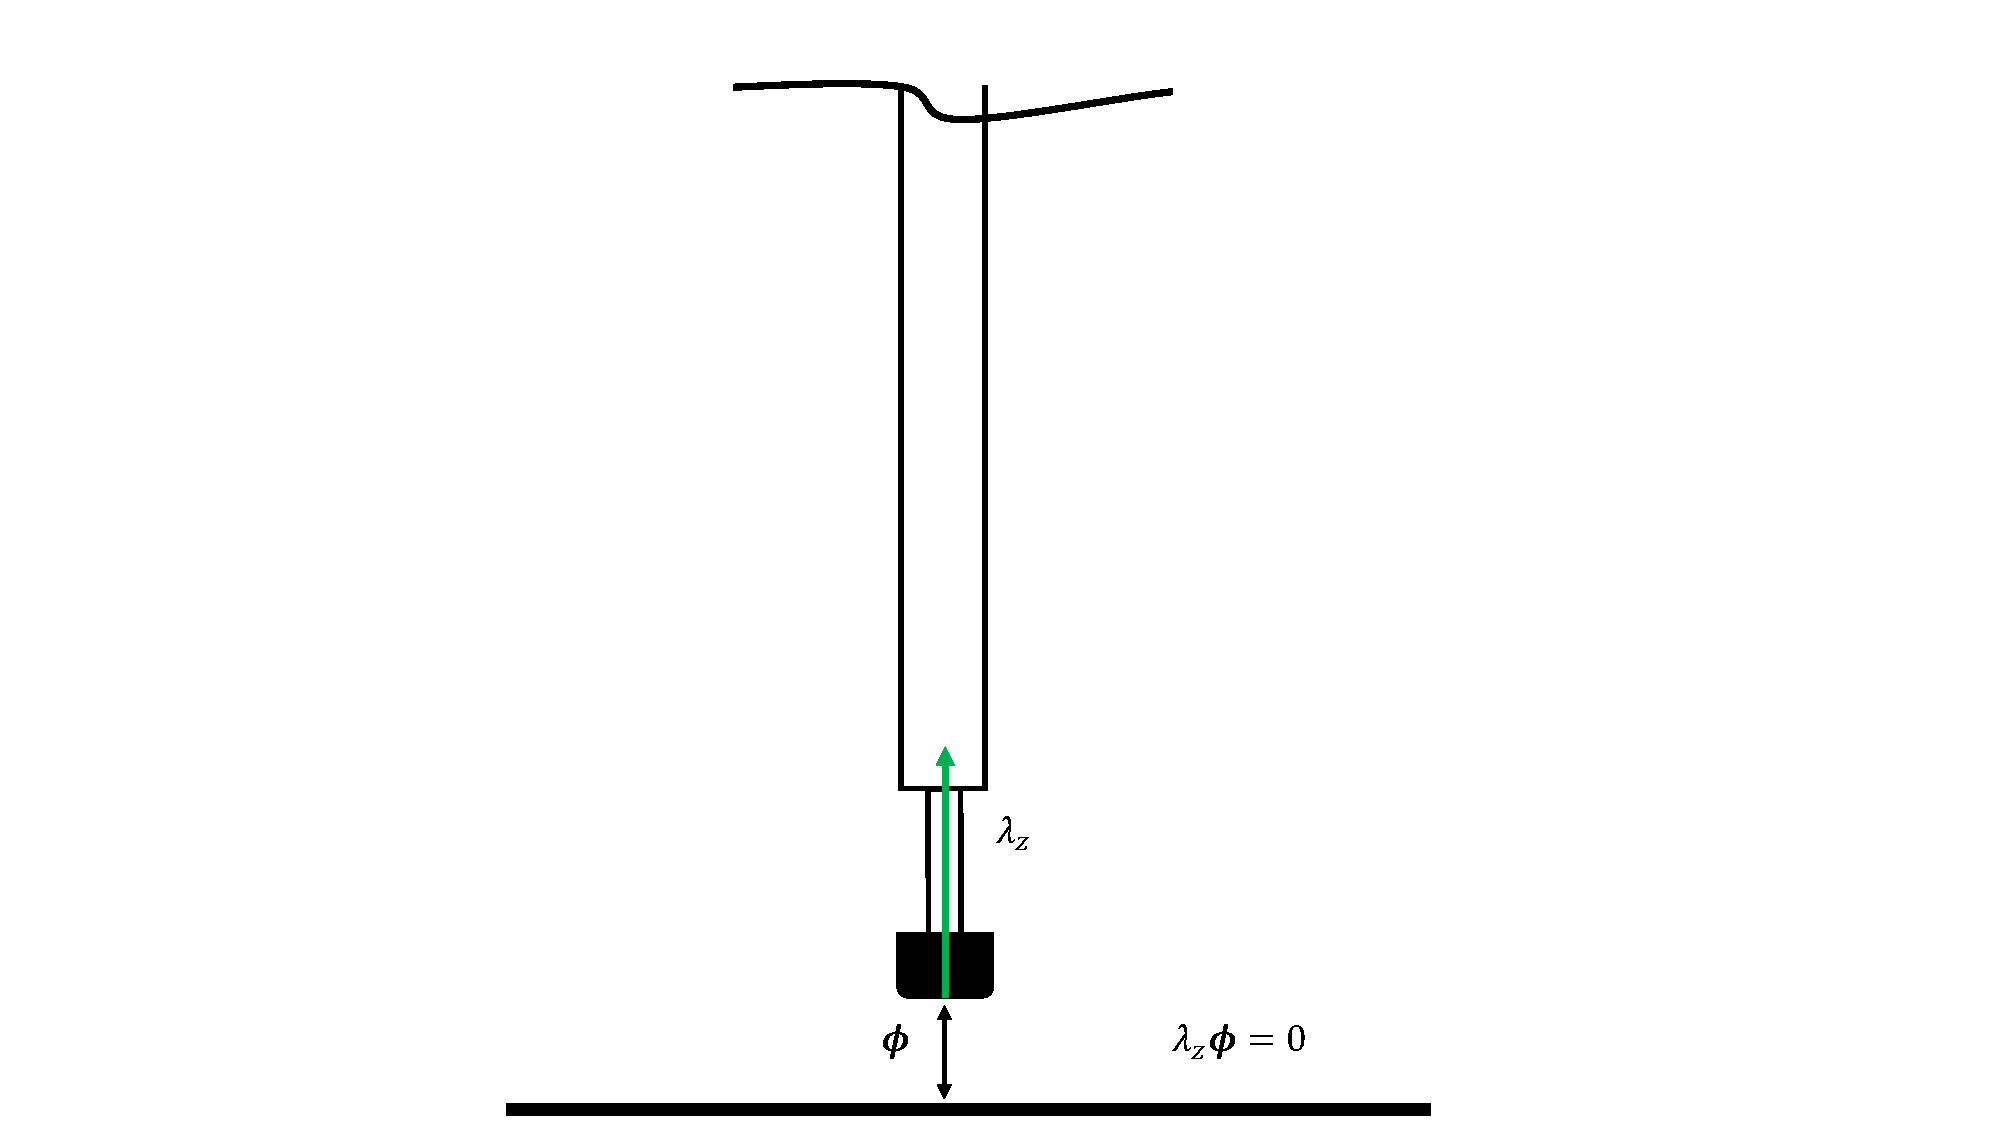
\includegraphics[width=\textwidth]{figs/grf}
            \caption{Figure showing a complementarity constraint for foot height and GRF. The foot height multiplied with the GRF in the z-direction must equal to zero. Thus, when the foot is in the air the GRF must equal to zero and vice versa to satisfy the constraint.}
            \label{fig:grf}
        \end{figure}
        
        To ensure that the horizontal ground reaction forces oppose the motion of slipping on the foot, the following two complementarity constraints were implemented:
        
        \begin{equation}
            \begin{split}
                (\gamma + \Psi(\bm{q}, \dot{\bm{q}}))^T \lambda^+_x = 0 \\
                (\gamma - \Psi(\bm{q}, \dot{\bm{q}}))^T \lambda^-_x = 0
            \end{split}
        \end{equation}
        
        %%%%%%%%%%%%%%%%%%%%%%%%%%%%%%%%%%%%%%%%%%%%%%%%%%%%%%%
        \subsubsection{Joint Angles}
        The EoM was generated using absolute angles. They equation generated by absolute angles are more simplified as to those generated by relative angles. These bounds are used to limit the motion and the velocity of the leg to feasible values. The bounds look as follow:
        
        \begin{equation}
            \begin{split}
                \textit{lower bound} &< \theta_{hip} < \textit{upper bound}\\
                \textit{lower bound} &< \omega_{hip} < \textit{upper bound}
            \end{split}
        \end{equation}
        
        Where the bounds were set according to the motor being used on the psychical system. These bounds can be found in more detail in Appendix \ref{app-a}.
        
        %%%%%%%%%%%%%%%%%%%%%%%%%%%%%%%%%%%%%%%%%%%%%%%%%%%%%%%%%%55
        \subsubsection{Start and Terminal Conditions}
        These constraints describe the conditions where the optimiser terminates the trajectories. The constraints were varied depending on the optimisation task being preformed and is described in the relevant chapters. The equations bellow describe the trajectory scheme that was used throughout the project:
        \begin{itemize}
            \item Acceleration Trajectories:
            \begin{itemize}
                \item Start at rest:
                \begin{equation}
                    \begin{split}
                        \bm{q}_0(1) &= \bm{q}_{rest} \\
                        \dot{\bm{q}}_0(1) &= \dot{\bm{q}}_{rest} = 0
                    \end{split}
                \end{equation}
                %%%%%
                \item Terminate at the apex of the steady-state trajectory:
                \begin{equation} \label{eq:terminal_accel}
                    \begin{split}
                        \bm{q}_0(N) &= \bm{q}_0(1)_{steady-state} \\
                        \dot{\bm{q}}_0(N) &= \dot{\bm{q}}_0(1)_{steady-state}
                    \end{split}
                \end{equation}
            \end{itemize}
            
            \item Steady-State Trajectory:
            \begin{itemize}
                \item Start at the apex of the trajectory:
                \begin{equation}
                    \begin{split}
                        \bm{q}_0(1) &= \bm{q}_0(1)_{steady-state} \\
                        \dot{\bm{q}}_0(1) &= \dot{\bm{q}}_0(1)_{steady-state} 
                    \end{split}
                \end{equation}
                %%%%%
                \item Terminate to enforce periodicity:
                   \begin{equation} \label{eq:terminal_ss}
                        \begin{split}
                            \bm{q}_0(N) &= \bm{q}_0(1) \\
                            \dot{\bm{q}}_0(N) &= \dot{\bm{q}}_0(1)
                        \end{split}
                    \end{equation}
            \end{itemize}
            
            \item Deceleration Trajectory:
            \begin{itemize}
                \item Start at the apex of steady-state trajectory:
                \begin{equation}
                    \begin{split}
                        \bm{q}_0(1) &= \bm{q}_0(1)_{steady-state} \\
                        \dot{\bm{q}}_0(1) &= \dot{\bm{q}}_0(1)_{steady-state}                     
                    \end{split}
                \end{equation}
                %%%%%
                \item Terminate at rest:
                \begin{equation} \label{eq:terminal_decel}
                    \begin{split}
                        \bm{q}_0(N) &= \bm{q}_{rest} \\
                        \dot{\bm{q}}_0(N) &= \dot{\bm{q}}_{rest} = 0
                    \end{split}
                \end{equation}            
            \end{itemize}
        \end{itemize}
        
        %%%%%%%%%%%%%%%%%%%%%%%%%%%%%%%%%%%%%%%%%%%%%%%%%%%%%%%%%%%%%%%55
        \subsubsection{Bounds}
        Bounds were enforced on all decision variables to restrict the search and reduce the problem size. The optimiser varies the varies the variables between the decision bounds until the set cost function is minimised.
        
        To ensure rapid motion, an upper bound was enforced on the total time allowed for the trajectory. It was implemented as follow:
        
        \begin{equation}
            \sum^N_{i=1}h(i) < T_{max}
        \end{equation}
    
        $T_{max}$ was obtained by manually reducing the value until the optimiser could no longer find a feasible solution.
        
        The ground reaction forces (GRF), $\lambda$, were bound to be less than $10m_{robot}g$, where $g$ is the the gravitational constant ($9.81 m/s^2$). This was done to limit the forces acting out on the ground to ensure that the mechanical system would not fail as a result of that.
    
        %%%%%%%%%%%%%%%%%%%%%%%%%%%%%%%%%%%%%%%%%%%%%%%%%%%%%%%%%55
        \subsubsection{Hard Stops for Prismatic Actuators} \label{Hard Stops}
        For prismatic actuators, hard stops are implemented to stop the optimiser from over over extending or over retracting the actuator. The following complimentary constraints are used:
        
        \begin{itemize}
            \item Minimum length hard stop:
            \begin{equation}
                \begin{split}
                    l(i) - l_{min} &= \alpha(i) \\
                    \alpha(i)*F_{HS}(i) &= 0                     
                \end{split}
            \end{equation}
            %%%%%
            \item Maximum length hard stop:
            \begin{equation}
                \begin{split}
                    l_{max} - l(i) &= \alpha(i) \\
                    \alpha(i)*F_{HS}(i) &= 0                     
                \end{split}
            \end{equation}          
        \end{itemize}
        
        Where $\alpha(n)$ is set to determine the actuator's length away from the minimum or maximum length allow for the actuator to retract and extend. It is then multiplied with a force ($F_{HS}$), which represents the actuator hitting its limits, and then set equal to zero. This complementary constrain forces the $F_{HS}$ to be applied when the actuator reaches it's limits, else it is zero.
        
        %%%%%%%%%%%%%%%%%%%%%%%%%%%%%%%%%%%%%%%%%%%%%%5
        \subsubsection{Solenoid Switching} \label{Sol Switching}
        Solenoids take a set amount of time, depending on solenoid being used, to switch from one state to another. To account for this, extra "bucket" nodes ($K$) were created to group a bunch of nodes ($i$), as is seen in Figure \ref{fig:switching}, to reduce the resolution of the prismatic force and preventing it form rapid extension and contraction. \textbf{UPDATE IMAGE}
       
        \begin{figure}[ht!]
            \centering
            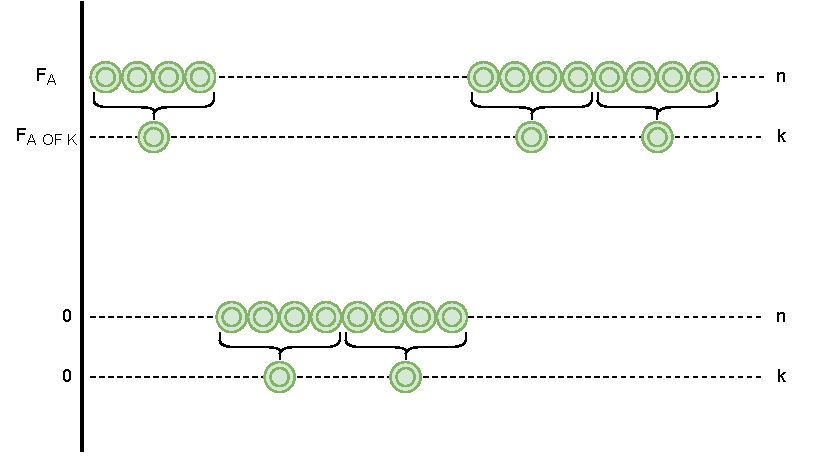
\includegraphics[width=\textwidth]{figs/switching}
            \caption{The graph shows a graphical representation of the nodes are grouped for solenoid switching}
            \label{fig:switching}
        \end{figure}
        
        Each bucket consists out of $N/K$ nodes. $K$ was chosen based on how much the prismatic actuator was expected to extend or retract and had to be a factor of $N$ to ensure that the bucket can be divided into equal amounts. Two force variables were generated, $F_A$ and $F_{\textit{A of K}}$, which consists out of $N$ and $K$ respectively, as shown below:
        
        \begin{equation}
            \begin{split}
                F_A(i), i \in(1, N) \\
                F_{\textit{A of K}}(k), k \in(1, K)
            \end{split}
        \end{equation}
        
        The following constrain ensured that the force value, $F_A$, at any $i^{th}$ node point was equal to force value, $F_{\textit{A of K}}$, of the bucket it was a part of: 

        \begin{equation}
            F_A(i) = F_{\textit{A of K}}(k), i \in(\frac{N(k-1)}{K}, \frac{Nk}{K}), k \in(1, K)
        \end{equation}
        
        This method allows for the numbers of nodes used to be kept high to ensure that the trajectory is smooth, while ensuring that the delay of the solenoid switching states was accounted for.
        
        %%%%%%%%%%%%%%%%%%%%%%%%%%%%%%%%%%%%%%%%%%%%%%%%
        \subsubsection{Bang-Bang Dynamics} \label{Bang-Bang}
        To make these trajectories realisable on a robotic system with pneumatic actuators, the bang-bang dynamics thereof should be accounted for. These constraints need to be applied to both the retraction and extension forces for the cylinder. These constrains were applied to the supplementary bucket force, $F_{\textit{A of K}}$, created before it was equated back to the force, $F_A$, acting in on the $i^{th}$ collection of nodes forming the bucket, as previously explained in Section \ref{Sol Switching}. The complimentary constraints used look as follow:
        
        \begin{equation}
            \begin{split}
                1-F_{\textit{A of K,extend}}(k) = \alpha(k) \\
                \alpha(k) * F_{\textit{A of K,extend}}(k) = 0            
            \end{split}
        \end{equation}
        
        \begin{equation}
            \begin{split}
                1-F_{\textit{A of K,retract}}(k) = \alpha(k) \\
                \alpha(k) * F_{\textit{A of K,retract}}(k) = 0            
            \end{split}
        \end{equation}
        
        These constraints force $F_{\textit{A of K}}$ (the actuator force) to either "on" or "off". To satisfy these constraints one of the products need to be zero. This means as soon as a force is applied $\alpha(k)$ should be zero which forces $F_{\textit{A of K}}(k)$ to be $1$, so that $\alpha(k) = 1-F_{\textit{A of K}}(k)$ is equal to zero.
        
        \begin{equation}
            F_{\textit{A of K,extend}}*F_{\textit{A of K,retract}} = 0
        \end{equation}
        
        %%%%%%%%%%%%%%%%%%%%%%%%%%%%%%%%%%%%%%%%%%%%%%%%%
        \subsubsection{Motor Model}
        In order to make the trajectories realisable on an actual robotics system, the motor model needs to be accounted for. The motor was implemented using a linear motor power model, taking into account the stall torque and no load speed specifications for the used motors. The follow constraints were implemented:
        
        \begin{equation}
            -\tau_{max} - \frac{\tau_{max}}{\omega_{max}}\omega(i) \leq \tau(i) \leq \tau_{max} - \frac{\tau_{max}}{\omega_{max}}\omega(i) 
        \end{equation}
        
        Where $\tau_{max}$ is the stall torque and $\omega_{max}$ is the no load speed of the motor.
        
        %%%%%%%%%%%%%%%%%%%%%%%%%%%%%%%%%%%%%%%%%%%%%%%%%
        \subsubsection{Fixed Contact Constraints}
        \textbf{Will see if this is used}
        
    \section{Controller Design}